\documentclass[10pt, fullpage, a4paper, titlepage]{article}
\usepackage{graphicx, latexsym}
\usepackage{subfigure}
\usepackage{setspace}
\usepackage{amssymb, amsmath, amsthm}
\usepackage{bm}
\usepackage{epstopdf}
\usepackage{rotating} %used for \sidewaystable
\usepackage{apacite}
\usepackage{booktabs} %used for \toprule
\usepackage{multirow} %used for \multirow and \multicolumn
%\singlespacing
%\onehalfspacing
\doublespacing

\begin{document}


\begin{figure}[h]
	\begin{center}
		\resizebox{\textwidth}{!}{
		\subfigure[Histogram]{
		\label{histogram:a}
	  			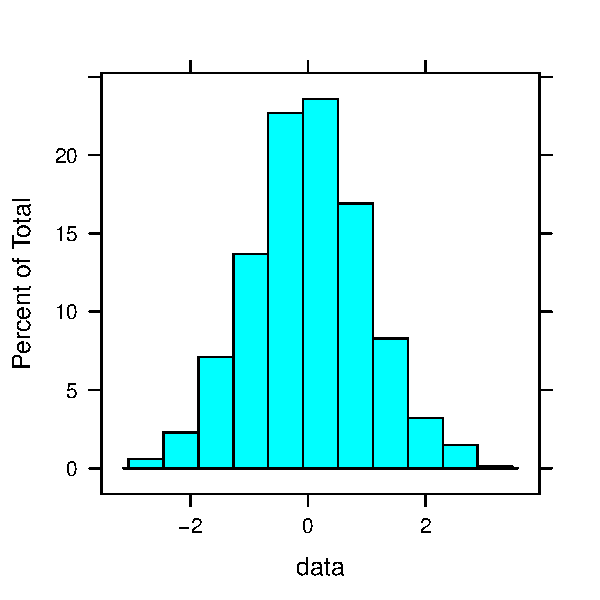
\includegraphics[scale=.5]{Plots/a.pdf}
	                 }
			\subfigure[Densityplot]{
 		        \label{densityplot:b}
				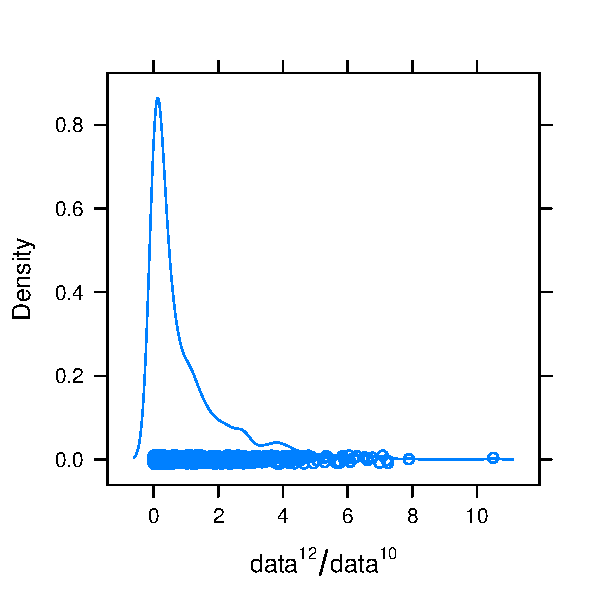
\includegraphics[scale=.5]{Plots/b.pdf}
		        }
		}\\ 	%  ------- End of the first row ----------------------%
		\resizebox{\textwidth}{!}{
			 \subfigure[Stripplot]{
  		        \label{stripplot:c}
	 			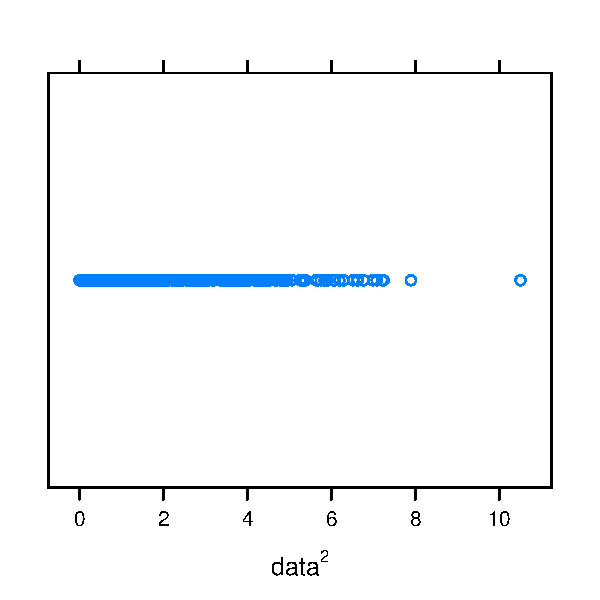
\includegraphics[scale=.5]{Plots/c.pdf}
			 }
			 \subfigure[Boxplot]{%
 		        \label{boxplot:d}
				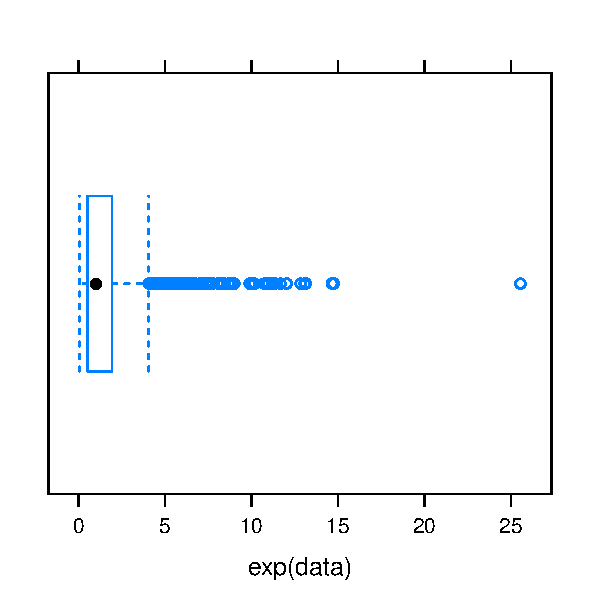
\includegraphics[scale=.5]{Plots/d.pdf}
			 }
		}
	\end{center}
	\caption{Different plots of the same data, sometimes transformed. No particular objective other than it being an exercise.}
	\label{Fig1}
\end{figure}

% latex table generated in R 3.2.2 by xtable 1.8-0 package
% Mon Aug 22 08:23:45 2016
\begin{table}[h!]
	\centering
	\caption{The same data, but now in a table. Only the first nine rows are displayed.}
	\begin{tabular}{rrrrr}
  		\hline
		 & data & squared1 & squared2 & exponent \\ 
		\hline
		1 & -0.56 & 0.31 & 0.31 & 0.57 \\ 
  		2 & -0.23 & 0.05 & 0.05 & 0.79 \\ 
		3 & 1.56 & 2.43 & 2.43 & 4.75 \\ 
  		4 & 0.07 & 0.00 & 0.00 & 1.07 \\ 
  		5 & 0.13 & 0.02 & 0.02 & 1.14 \\ 
  		6 & 1.72 & 2.94 & 2.94 & 5.56 \\ 
  		7 & 0.46 & 0.21 & 0.21 & 1.59 \\ 
  		8 & -1.27 & 1.60 & 1.60 & 0.28 \\ 
  		9 & -0.69 & 0.47 & 0.47 & 0.50 \\ 
		\hline
	\end{tabular}
\end{table}


\end{document}